\documentclass[14pt,a4paper]{scrartcl}
\usepackage[utf8]{inputenc}
\usepackage[english,russian]{babel}
\usepackage{indentfirst}
\usepackage{misccorr}
\usepackage{graphicx}
\usepackage{amsmath}
\usepackage{amsfonts}
\usepackage{graphicx}
\usepackage{float}
\usepackage[cache=false]{minted}

\graphicspath{{img/}}

\begin{document}
	\begin{center}
		МОСКОВСКИЙ ГОСУДАРСТВЕННЫЙ УНИВЕРСИТЕТ
		\\
		им. М.В. Ломоносова
		\\
		\bigskip
		Факультет Вычислительной Математики и Кибернетики
		\\
		\bigskip
		Кафедра Исследования Операций
	\end{center}
	\begin{figure}[h]
		\centering
		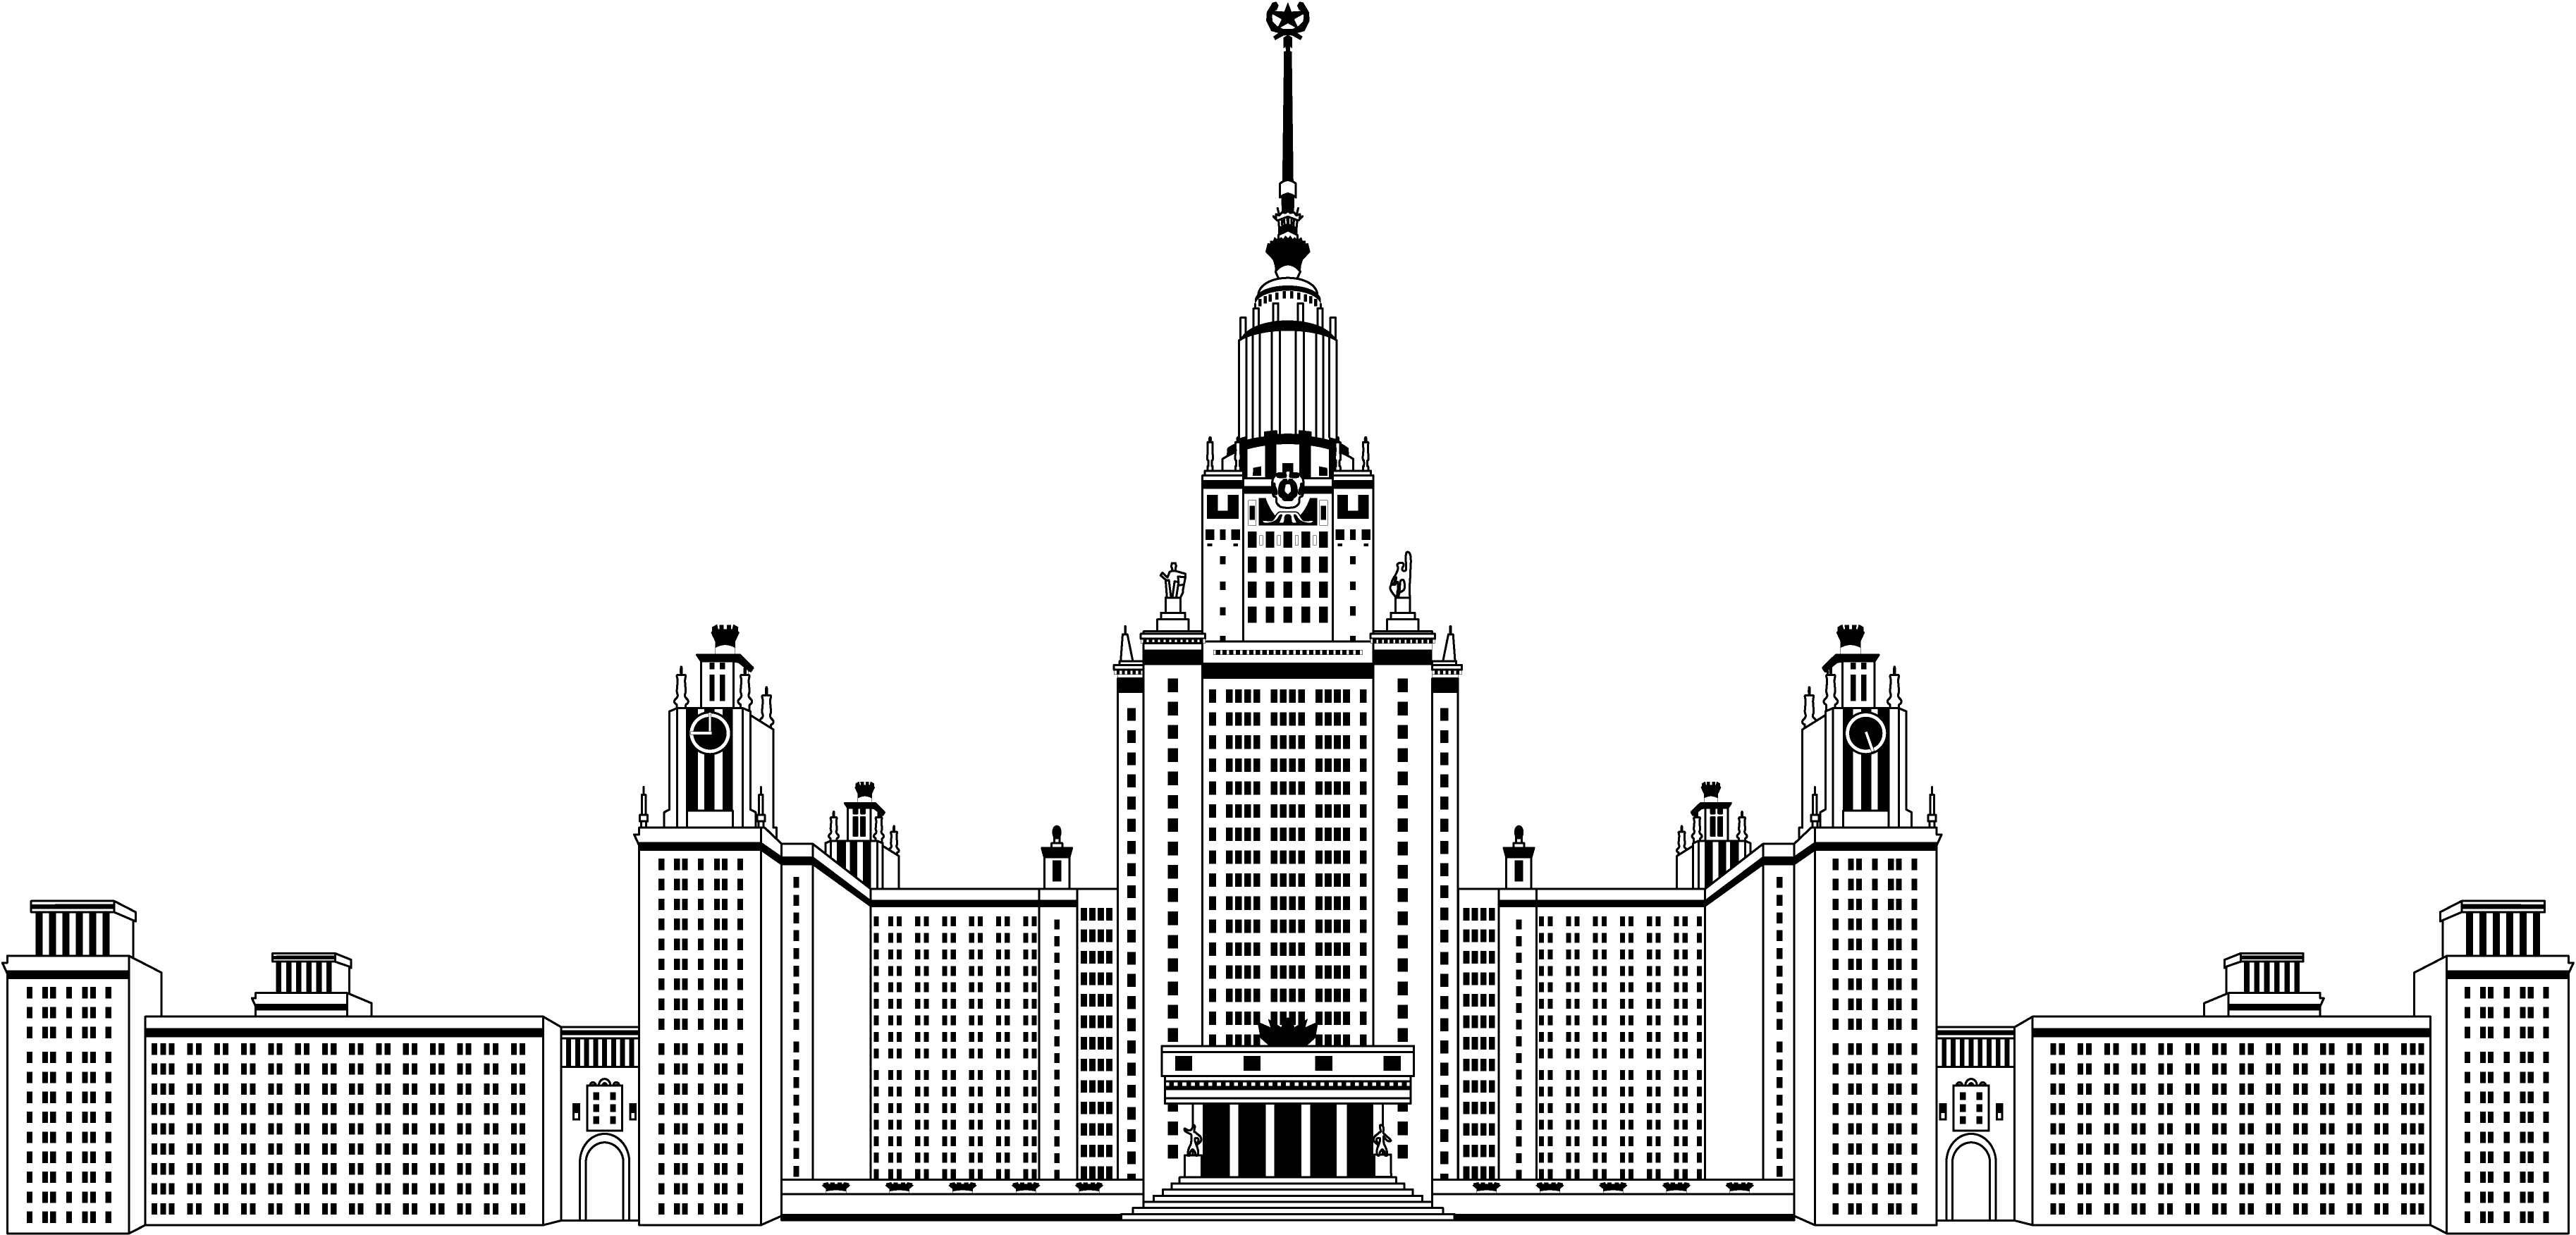
\includegraphics[width=0.8\linewidth]{MSU}
	\end{figure}
	\begin{center}
		Отчет по практическому заданию по курсу
		\\
		Пакеты Прикладных Программ
		\\
		\bigskip
		Задача о коммивояжере.
		\\
		Метод отжига.
	\end{center}
	\bigskip
	\begin{flushright}
		Студент 412 группы
		\\
		Денисов Никита
	\end{flushright}
	\vfill
	\begin{center}
		Москва 2021
	\end{center}
	\newpage
	\tableofcontents
	\newpage
	\section{Постановка задачи}
	\subsection{Общие сведения}
	\begin{flushleft}
		Задача коммивояжёра --- задача комбинаторной оптимизации, заключающаяся в поиске самого выгодного маршрута, проходящего через указанные города хотя бы по одному разу с последующим возвращением в исходный пункт.В условиях задачи указываются критерий выгодности маршрута (кратчайший, самый дешёвый, совокупный критерий и тому подобное) и соответствующие матрицы расстояний, стоимости и т.д.
		\\
		Представим задачу в виде математической модели. Задачу коммивояжёра можно представить в виде модели на графе, то есть, используя вершины и ребра между ними. Таким образом, вершины графа соответствуют городам, а рёбра $(i, j)$ между вершинами $i$ и $j$ --- пути сообщения между этими городами. Каждому ребру $(i, j)$ сопоставляется критерий качества маршрута $c_{ij}$ --- расстояние между городами, стоимость поездки или необходимое время.
		\\
		Задачи о коммивояжёре можно разделить на два класса:
		\\
		\begin{itemize}
			\item симметрическая задача --- все пары ребер между одними и теми же вершинами имеют одинаковую длину, то есть, для ребра $(i, j)$ одинаковы длины $c_{ij} = c_{ji}$.
			\item ассиметрическая задача --- моделируется ориентированным графом и равенство $c_{ij} = c_{ji}$, вообще говоря, не выполняется. Следовательно, количество возможных маршрутов вдвое больше, чем в симметрическом случае.
		\end{itemize}
	\end{flushleft}
		\begin{figure}[H]
			\centering
			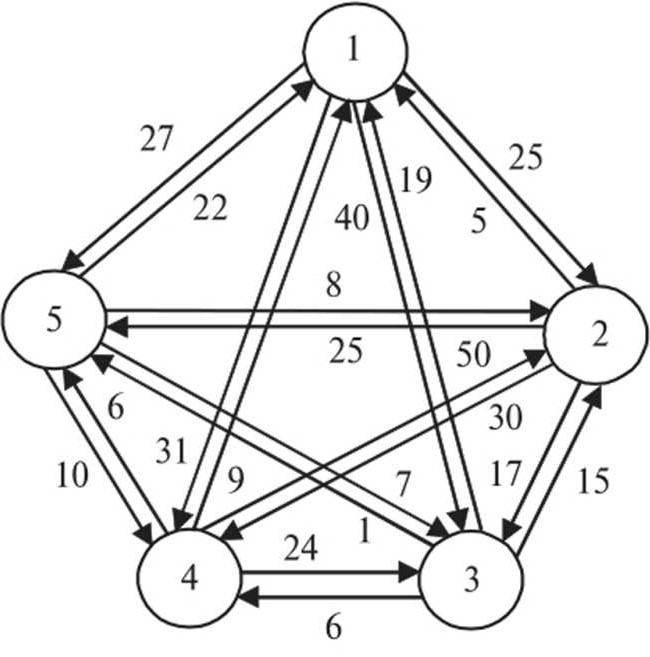
\includegraphics[width=0.5\linewidth]{task_example}
			\caption{Визуализация ассиметрической задачи}
		\end{figure}
	\begin{flushleft}
		Задача о коммивояжёре называется метрической,  если относительно длин ребер выполняется неравенство треугольника. Условно говоря, в таких задачах обходные пути длиннее прямых, то есть ребро от вершины $i$ до вершины $j$ никогда не бывает длиннее пути через промежуточную вершину $k$: $c_{ij} \leq c_{ik} + c_{kj}$.
	\end{flushleft}
	\subsection{Формулировка в виде задачи дискретной оптимизации}
	\begin{flushleft}
		Одним из подходов к решению задачи является формулировка её в виде задачи дискретной оптимизации, при этом решения представляются в виде переменных, а связи --- в виде отношений неравенства между ними. Таким образом, возможно несколько вариантов. Например, симметричную задачу можно представить в виде множества ребер $V$.Каждому ребру $(i, j)$ сопоставляется двоичная переменна $x_{ij} \in \{0, 1\}$, равная 1, если ребро принадлежит маршруту, и 0 --- в противном случае. Произвольный маршрут можно представить в виде значений множества переменных принадлежности, но не каждое такое множество определяет маршрут. Условием того, что значения множества переменных определяют маршрут, являются описанные далее линейные неравенства.
		\\
		\bigskip
		Каждая вершина должна сообщаться через пару ребер с остальным вершинам, то есть, через входное и выходное ребро:
		$$\forall i \in V: \sum\limits_{j \in V \backslash\{i\}} x_{ij} = 2 \eqno{(1)}$$
		\\
		В сумме каждое слагаемое $x_{ij}$ равно или 1 (принадлежит маршруту) или 0 (не принадлежит). То есть, полученная сумма равна количеству ребер в маршруте, имеющих вершину $i$ на одном из концов. Она равна 2, так как каждая вершина имеет входное и выходное ребро. В приведенном рядом рисунке вершина $i$ показана с входным и выходными ребрами, а ребра маршрута обозначены толстыми линиями. Рядом с ребрами указаны длины $x_{ij}$, прилагаемые к указанной выше сумме.
		\\
		\bigskip
		Описанные ранее условия кратности выполняются не только маршрутами, но и значениями переменных, соответствующих отдельным циклам, где каждая вершина принадлежит лишь одному циклу. Чтобы избежать подобных случаев, должны выполняться так называемые неравенства циклов (или условия устранения подмаршрутов), которые были определены Данцигом, Фалкерсоном и Джонсоном в 1954 году под названием условия петель. Этими неравенствами определялось дополнительное условие того, что каждое множество вершин $S \subset V$ является либо пустым, либо содержит все вершины, сочетающееся с остальным вершинам через минимум два ребра:
		$$\sum\limits_{i \in S, j \notin S} x_{ij} \geq 2 \eqno{(2)}$$
		для всех множеств вершин $S$, где $1 \leq |S| \leq |V| - 1$. Эта сумма равна сумме длин ребер маршрута между вершиной $i \in S$ и вершиной $j \notin S$. Чтобы устранить лишние неравенства, можно ограничиться множествами вершин $S$ с минимум двумя и максимум $|V| - 2$ вершинами. Количество неравенств устранения циклов согласно Данцигу, Фалкерсону и Джонсону равняется $2^n - 2(n - 1)$.
		\\
		Наконец, приведем окончательную постановку задачи:
		$$\sum\limits_{i \in V} \sum\limits_{j \in V \backslash \{i\}} c_{ij}x_{ij} \rightarrow min$$
		\begin{center}
			$x$ удовлетворяет $(1), (2)$
		\end{center}
		$$x_{ij} \in \{0, 1\}$$
	\end{flushleft}
	\section{Решение поставленной задачи}
	\subsection{Алгоритм имитации отжига. Описание.}
	\begin{flushleft}
	Алгоритм основывается на имитации физического процесса, который происходит при кристаллизации вещества, в том числе при отжиге металлов. Предполагается, что атомы уже выстроились в кристаллическую решётку, но ещё допустимы переходы отдельных атомов из одной ячейки в другую. Предполагается, что процесс протекает при постепенно понижающейся температуре. Переход атома из одной ячейки в другую происходит с некоторой вероятностью, причём вероятность уменьшается с понижением температуры. Устойчивая кристаллическая решётка соответствует минимуму энергии атомов, поэтому атом либо переходит в состояние с меньшим уровнем энергии, либо остаётся на месте.
	\\
	При помощи моделирования такого процесса ищется такая точка или множество точек, на котором достигается минимум некоторой числовой функции $F(\overline{x})$, где $\overline{x} = (x_1, \ldots, x_m) \in X$. Решение ищется последовательным вычислением точек $\overline{x_0}, \overline{x_1}, \ldots,$ пространства $X$;каждая точка, начиная с $\overline{x_1}$, «претендует» на то, чтобы лучше предыдущих приближать решение. Алгоритм принимает точку $\overline{x_0}$ как исходные данные. На каждом шаге алгоритм вычисляет новую точку и понижает значение величины (изначально положительной), понимаемой как «температура». Алгоритм останавливается по достижении точки, которая оказывается при температуре ноль.
	\\
	Точка $\overline{x_{i+1}}$ по алгоритму получается на основе текущей точки $\overline{x_{i}}$ следующим образом. К точке $\overline{x_{i}}$ применяется оператор $A$, который случайным образом модифицирует соответствующую точку, в результате чего получается новая точка $\overline{x^{*}}$. Точка $\overline{x^{*}}$ становится точкой $\overline{x_{i+1}}$ с вероятностью $P(\overline{x^{*}}, \overline{x_{i+1}})$, которая вычисляется в соответствии с распределением Гиббса:
		\begin{equation*}
			P(\overline{x^{*}} \rightarrow \overline{x_{i+1}} | \overline{x_{i}}) = 
				\begin{cases}
				1 &\text{,$F(\overline{x^{*}}) - F(\overline{x_{i}}) < 0$}\\
				exp(-\frac{F(\overline{x^{*}}) - F(\overline{x_{i}})}{Q_{i}}) &\text{,$F(\overline{x^{*}}) - F(\overline{x_{i}}) \geq 0$}
				\end{cases}
				\eqno{(3)}
		\end{equation*}
	Здесь $Q_{i} > 0$ --- элементы произвольной, убывающей, сходящейся к нулю положительной последовательности, которая задаёт аналог падающей температуры в кристалле. Скорость убывания и закон убывания задаются пользователем.
		\begin{figure}[H]
			\centering
			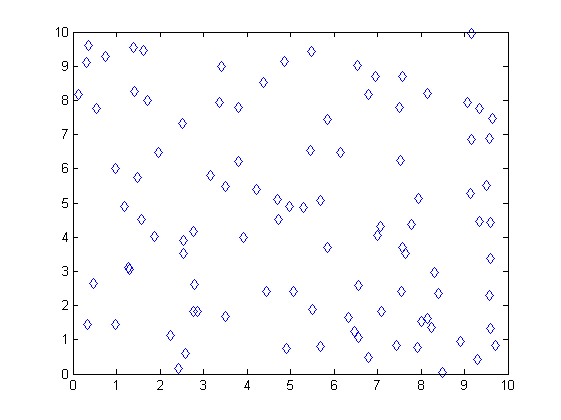
\includegraphics[width=0.7\linewidth]{cities2d}
			\caption{Множество городов на плоскости}
		\end{figure}
	\bigskip
	Теперь сформулируем алгоритм конкретно для нашей задачи. Множеством городов будем считать множество точек на плоскости (Рис. 2). Тогда критерий выгодности маршрута - расстояние между двумя городами: $c_{ij} = \sqrt{(x_j - x_i)^2 + (y_j - y_i)^2}$. Пускай $C$ --- множество всех городов, а $|C|$ --- их количество. Введем целевую функцию, которую мы будем минимизировать:
	$$E_{i} = E(x^{i}) = \sum\limits_{1}^{|C|-1} c_{k \: k+1} + \sqrt{(x_{|C|} - x_1)^2 + (y_{|C|} - y_i)^2} \eqno{(4)}$$
	Также, необходима фунция убывания температуры. Единственное требование к ней --- она должна генерировать положительную и сходящуюся к нулю последовательность. Остановим свой выбор на линейной функции:
	$$Q_{i} = \frac{T_{max}}{i} \eqno{(5)}$$
	Критиерий продолжения итераций:
	$$Q_{i} \geq T_{min} \eqno{(6)}$$
	Далее, для простоты, будем считать, что города занумерованы натуральными числами $1, 2, \ldots$. Распишем шаги алгоритма:
		\begin{enumerate}
			\item Случайным образом генерируем начальную последовательность городов --- вектор неповторяющихся натуральных чисел $x^{0}$ (номера городов). Вычисляем целевую функцию $E_{0}$.
			\item Очередной вектор $x^{i}, i = 1, 2, \ldots$ получаем перестановкой двух случайных компонент вектора $x^{i-1}$. Вычисляем целевую функцию $E_{i}$. Вычисляем вероятность $P$ перехода к вектору $x^{i}$, используя формулы (3), (5). Если она равна 1 --- принимаем вектор $x^{i}$. Иначе генерируем случайное число $\xi \in [0, 1]$. Если $\xi \leq P$, то принимаем вектор $x^{i}$, иначеоставляем текущий вектор и повторяем итерации.
			\item Продолжаем итерации (пункт 2), пока выполняется условие (6). 
		\end{enumerate}
	\end{flushleft}
	\subsection{Обоснование корректности алгоритма}
	\begin{flushleft}
		Алгоритм имитации отжига является эвристическим и описывает реальный физический процесс, происходящий в металлах при закалке. Алгоритм имитации отжига похож на градиентный спуск, но за счёт случайности выбора промежуточной точки должен попадать в локальные минимумы реже, чем градиентный спуск. Алгоритм имитации отжига не гарантирует нахождения минимума функции, однако при правильной политике генерации случайной точки в пространстве $X$, как правило, происходит улучшение начального приближения. Подбор функции генерации температуры (то есть убывающей последовательности) может улучшить скорость работы алгоритма и его робастность.
	\end{flushleft}
	\section{Программная реализация алгоритма}
	\subsection{Краткое описание}
	\begin{flushleft}
		Алгоритм имитации отжига для задачи коммивояжёра реализован на языке Python 3 в виде класса. Такоя подход позволяет легко импортировать код в другие проекты. Экземпляр класса инициализиуется набором городов, который может быть задан списком, массивом, записан в файле или сгенерирован случайно (подходит для демонстрации работы программы). На этапе инициализации есть базовая проверка типов, чтобы исключить основные ошибки ввода. Все поля класса являются открытыми, а единственный открытый метод, доступный пользователю --- OptimizeRoute(), в котором и происходят итерации алгоритма. Вспомогательные вычисления, а именно подсчет вероятности, генерация нового вектора, реазилованы в закрытых методах класса. Реализована простейшая функция убывания температуры, а именно $\frac{T_{max}}{i}$, где $i$ --- номер итерации. Также реализована возможность early stopping --- максимальное число итераций без улучшения целевой функции. Данное число рассчитывается как $T_{max}*(cities \; count)*\frac{cities \; count - 1}{2}$, то произведение максимальной температуры и количества всевозмодных уникальных пар городов. Такой подход позволяет сократить время работы программы без потери точности и робастности оптимизации. На рисунке ниже представлена визуализация результата работы алгоритма.
	\end{flushleft}
	\subsection{Листинг программы}
	\begin{minted}
	[
	frame = lines,
	framesep  = 2mm,
	baselinestretch = 1.2,
	bgcolor = white,
	fontsize = \small,
	linenos,
	breaklines, 
	breakautoindent=true
	]
	{python}
	import numpy as np
	import math
	import matplotlib.pyplot as plt
	import io
	
	class TSP():
	def __init__(self, cities_input = 50):
	if isinstance(cities_input, int):
	if cities_input >= 2:
	self.cities = np.random.uniform(0.0, 1.0, (2, cities_input))*10 #cities[0] - координата X, cities[1] - координата Y
	else:
	raise ValueError("Неправильное количество городов. Их должно быть больше двух.")
	
	elif isinstance(cities_input, list):
	try:
	self.cities = np.array(cities_input)
	except:
	raise ValueError("Проверьте данные. Списиок координат должен быть двумерным и содержать одинковое число (>= 2) координат X и Y.")
	
	elif isinstance(cities_input, np.ndarray):
	if cities_input.shape[0] == 2 and cities_input.shape[1] >= 2:
	self.cities = cities_input.copy()
	else:
	raise ValueError("Проверьте данные. Массив координат должен быть двумерным и содержать одинковое число (>= 2) координат X и Y.")
	
	elif isinstance(cities_input, io.IOBase):
	cities_x = list(map(float, cities_input.readline().split()))
	cities_y = list(map(float, cities_input.readline().split()))
	if len(cities_x) != len(cities_y):
	raise ValueError(f"Количество координат по X и по Y должно совпадать.\nКоординат X: {len(cities_x)}, координат Y: {len(cities_y)}")
	self.cities = np.array([cities_x, cities_y], dtype = np.float_)
	
	else:
	raise ValueError("Неверный формат входных данных. Возможные форматы: int, list, NumPy ndarray, file.")
	
	self.start_point = np.array(list(range(1, self.cities.shape[1] + 1)))
	np.random.shuffle(self.start_point)
	self.T_max = 1000
	self.T_min = 0.01
	self.max_iter_no_change = self.T_max*self.cities.shape[1]*(self.cities.shape[1] - 1)/2
	
	def __objective_function(self, cities_order): #целевая функция суммарного расстояния между текущей последовательностью городов (закрытый метод класса)
	distance = 0.0
	cities_order = np.append(cities_order, cities_order[0 : 1])
	for i in range(cities_order.shape[0] - 1):
	prev_city = cities_order[i] - 1
	next_city = cities_order[i + 1] - 1
	distance += ((self.cities[0, next_city] - self.cities[0, prev_city])**2 + (self.cities[1, next_city] - self.cities[1, prev_city])**2)**0.5
	return distance
	
	def __temperature_decrease(self, iteration): #функция убывания температуры (закрытый метод класса)
	return self.T_max/iteration
	
	def __generate_next_point(self, prev_point): #функция генерации следующей последовательности городов (закрытый метод класса)
	positions = np.arange(prev_point.shape[0])
	np.random.shuffle(positions)
	tmp_point = prev_point.copy()
	pos1 = positions[0]
	pos2 = positions[1]
	tmp_point[[pos1, pos2]] = tmp_point[[pos2, pos1]]
	return tmp_point
	
	def __get_probability(self, curr_point, next_point, iteration): #вычисляем вероятность принятия следующей последовательности гоордов (закрытый метод класса)
	if self.__objective_function(next_point) < self.__objective_function(curr_point):
	return 1.0
	else:
	return math.exp(-(self.__objective_function(next_point) - self.__objective_function(curr_point))/self.__temperature_decrease(iteration))
	
	def OptimizeRoute(self): #поиск оптимальной последовательности городов
	iteration = 1
	initial_point = self.start_point
	next_point = self.start_point.copy()
	iter_no_change = 0
	while self.__temperature_decrease(iteration) >= self.T_min:
	curr_point = next_point.copy()
	next_point = self.__generate_next_point(curr_point)
	probability = self.__get_probability(curr_point, next_point, iteration)
	if probability < 1.0:
	ksi = abs(np.random.uniform(-1.0, 1.0, 1)[0])
	if ksi >= probability:
	next_point = curr_point.copy()
	iter_no_change += 1
	if (curr_point != next_point).all():
	iter_no_change = 0
	if iter_no_change == self.max_iter_no_change:
	break
	iteration += 1
	self.end_point = next_point.copy()
	print("Конечная последовательность городов:", self.end_point)
	print("Исходное суммарное расстояние:", self.__objective_function(initial_point))
	print("Конечное суммарное расстояние:", self.__objective_function(self.end_point))
	initial_matrix = np.array([[self.cities[0, i - 1], self.cities[1, i - 1]] for i in initial_point]).T
	end_matrix = np.array([[self.cities[0, i - 1], self.cities[1, i - 1]] for i in self.end_point]).T
	fig = plt.figure(figsize = (12, 4), num = "TSP")
	plt.subplot(1, 3, 1, title = "Города")
	plt.scatter(self.cities[0], self.cities[1])
	plt.subplot(1, 3, 2, title = "Начальный путь")
	plt.scatter(self.cities[0], self.cities[1])
	plt.plot(initial_matrix[0], initial_matrix[1])
	plt.subplot(1, 3, 3, title = "Оптимальный путь")
	plt.scatter(self.cities[0], self.cities[1])
	plt.plot(end_matrix[0], end_matrix[1])
	plt.show()
	\end{minted}
	\subsection{Результат работы алгоритма}
	\begin{flushleft}
		На картинке ниже изображен процесс и результат работы алгоритма имитации отжига для задачи коммивояжёра: набор городов на плоскости, начальная последовательность городов и финальная, то есть оптимальная, последовательность городов.
		\begin{figure}[H]
			\centering
			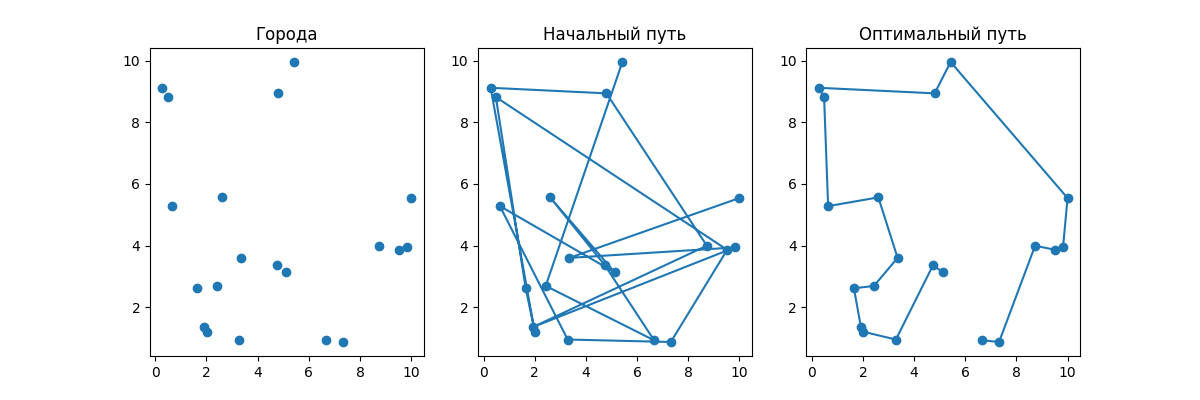
\includegraphics[width=1.0\linewidth]{TSP}
			\caption{Визуализация работы алгоритма}
		\end{figure}
	\end{flushleft}
	\subsection{Время работы алгоритма}
	\begin{flushleft}
		В резульате некоторого количества запусков алгоритма с разным количеством городов было получено, что зависимость времени работы программы от количества городов находится между $O(n)$ и $O(\ln(n))$, но всё же, ближе к линейной. Ниже приведена визуализация результатов исследования времени работы программы.
		\begin{figure}[H]
			\centering
			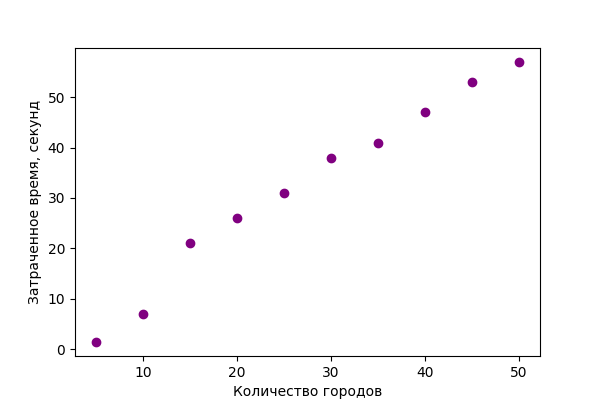
\includegraphics[width=1.0\linewidth]{Elapsed_time}
			\caption{Зависимость времени работы от количества городов}
		\end{figure}
	\end{flushleft}
\end{document}